\chapter{Overall description}

\section{Product perspective}

The Students\&Companies (S\&C) platform serves as a matchmaking hub for university students seeking internships and companies offering them.
It streamlines the process by matching student experiences, skills, and attitudes, with internships defined by specific projects, responsibilities, technologies, and benefits like mentorship and training.
The platform is actively used by students to browse and apply for internships, while also supporting companies in showcasing available positions.

S\&C includes an intelligent recommendation system to notify students of relevant opportunities and inform companies about suitable candidates, employing statistical analyses.
Additionally, it facilitates the interview and selection process, offering tools for collecting candidate responses, in the form of custom questionnaires.

The platform gathers feedback from both students and companies, in order to better feed the recommendation system.
Furthermore, it provides data-driven suggestions to enhance CVs and project descriptions.

Universities also engage with S\&C to oversee internship progress, handle complaints, and, if necessary, address issues that may require intervention.

\subsection{Scenarios}

\begin{enumerate}[label=\textbf{S\arabic* -}]
    \item \textbf{Signing up and logging in -}
    User Marco opens the platform and starts the sign-up procedure.
    He fills in the required information and completes the sign-up process.
    Then he logs out to make sure everything went smoothly, and a few seconds later, he logs in back again using the same credentials.
    \item \textbf{Filling in personal information -}
    Maria logs into the platform and accesses the profile section.
    She fills in the personal data fields, such as contact details, degree program and competence skills.
    After completing the desired fields, she clicks the "Save" button, and the system confirms that her information has been successfully updated.
    \item \textbf{Uploading the CV -}
    Luca decides to upload his CV, to be ready to apply for internship opportunities.
    He goes to the "Upload CV" section, selects the PDF file from his computer, and clicks "Upload".
    The system verifies the file validity and confirms the upload.
    Luca now has his CV associated with his profile, ready to be included with applications.
    \item \textbf{Creating an internship project advertisement -}
    A consulting firm logs into the platform to publish a new internship advertisement.
    Anna, the recruitment officer, fills in the required fields in the creation form, including the project description, required skills, and internship duration.
    After verifying the details, Anna selects “Publish”.
    The system confirms the publication, and the advertisement immediately becomes visible to students on the platform.
    \item \textbf{Notifying the availability of an internship -}
    Sara has set her preferences to receive notifications about internship opportunities in marketing.
    When a new company posts a relevant advertisement, the system automatically pushes a notification in her notification section.
    By opening this section page, Sara can quickly access the advertisement and decide whether to apply.
    \item \textbf{Selecting an internship project -}
    Alessandro is looking for an internship experience in computer engineering.
    He accesses the internship opportunities section and browses the available advertisements.
    When he finds an interesting offer at a startup, he views the details and decides to apply.
    The system confirms the submission of the application, and Alessandro receives a notification that the application was successfully sent.
    \item \textbf{Creating a custom questionnaire -}
    A technology company decides to filter candidates with a custom questionnaire on programming skills.
    Laura, the person in charge, accesses the platform, selects the option to create a questionnaire, and adds specific questions about algorithms and programming languages.
    After completing the questionnaire, Laura associates it with the internship advertisement, ready to be sent and completed by applicants.
    \item \textbf{Filling a questionnaire -}
    Martina is applying for an internship as a graphic designer at an advertising agency.
    During the application process, she is asked to complete a questionnaire evaluating her skills in graphic software like Photoshop and Illustrator.
    Martina answers all the questions and submits the questionnaire.
    The system confirms the submission, and Martina has completed her application.
    \item \textbf{Starting a new internship -}
    Giovanni successfully completes the selection process with the company.
    Once he has been confirmed, the system notifies both parties and updates the status to "Internship Started".
    Giovanni can now access the platform to monitor his progress during the internship.
    \item \textbf{Viewing internship information -}
    During her internship, Laura accesses the "Internship Information" section to monitor project details, including goals, deadlines, and her supervisor name.
    The platform allows her to view updates and track her progress, ensuring she meets the requirements and expectations of the internship.
    \item \textbf{Sending a complaint -}
    Paolo, a student on an internship, encounters issues with the support provided by the company.
    He decides to report the problem to the university through the platform.
    He accesses the complaints section, describes the issue, and submits the report.
    The system notifies the university administration, which reviews the case.
    After evaluating the situation, the university decides on the appropriate action, such as contacting the company for clarification or providing direct support to Paolo.
    \item \textbf{Receiving feedback -}
    After completing the internship, both the student and the company provide feedback about their experience.
    The student evaluates the company regarding working conditions, support received, and the relevance of the assigned activities, while the company provides feedback on the skills and effort demonstrated by the student.
    These feedback reports are collected by the platform and made available to the university for an overall evaluation of the internship experience.
\end{enumerate}

\subsection{Class diagram}

The UML class diagram below represents a high-level conceptual model of the software.

Due to the highly changing nature of the project, the UML may model objects that will not be implemented in the actual system.
Moreover, at this level, any reference to methods and other low-level details will not be included, as detailed in the design phase.

\begin{figure}[H]
    \centering
    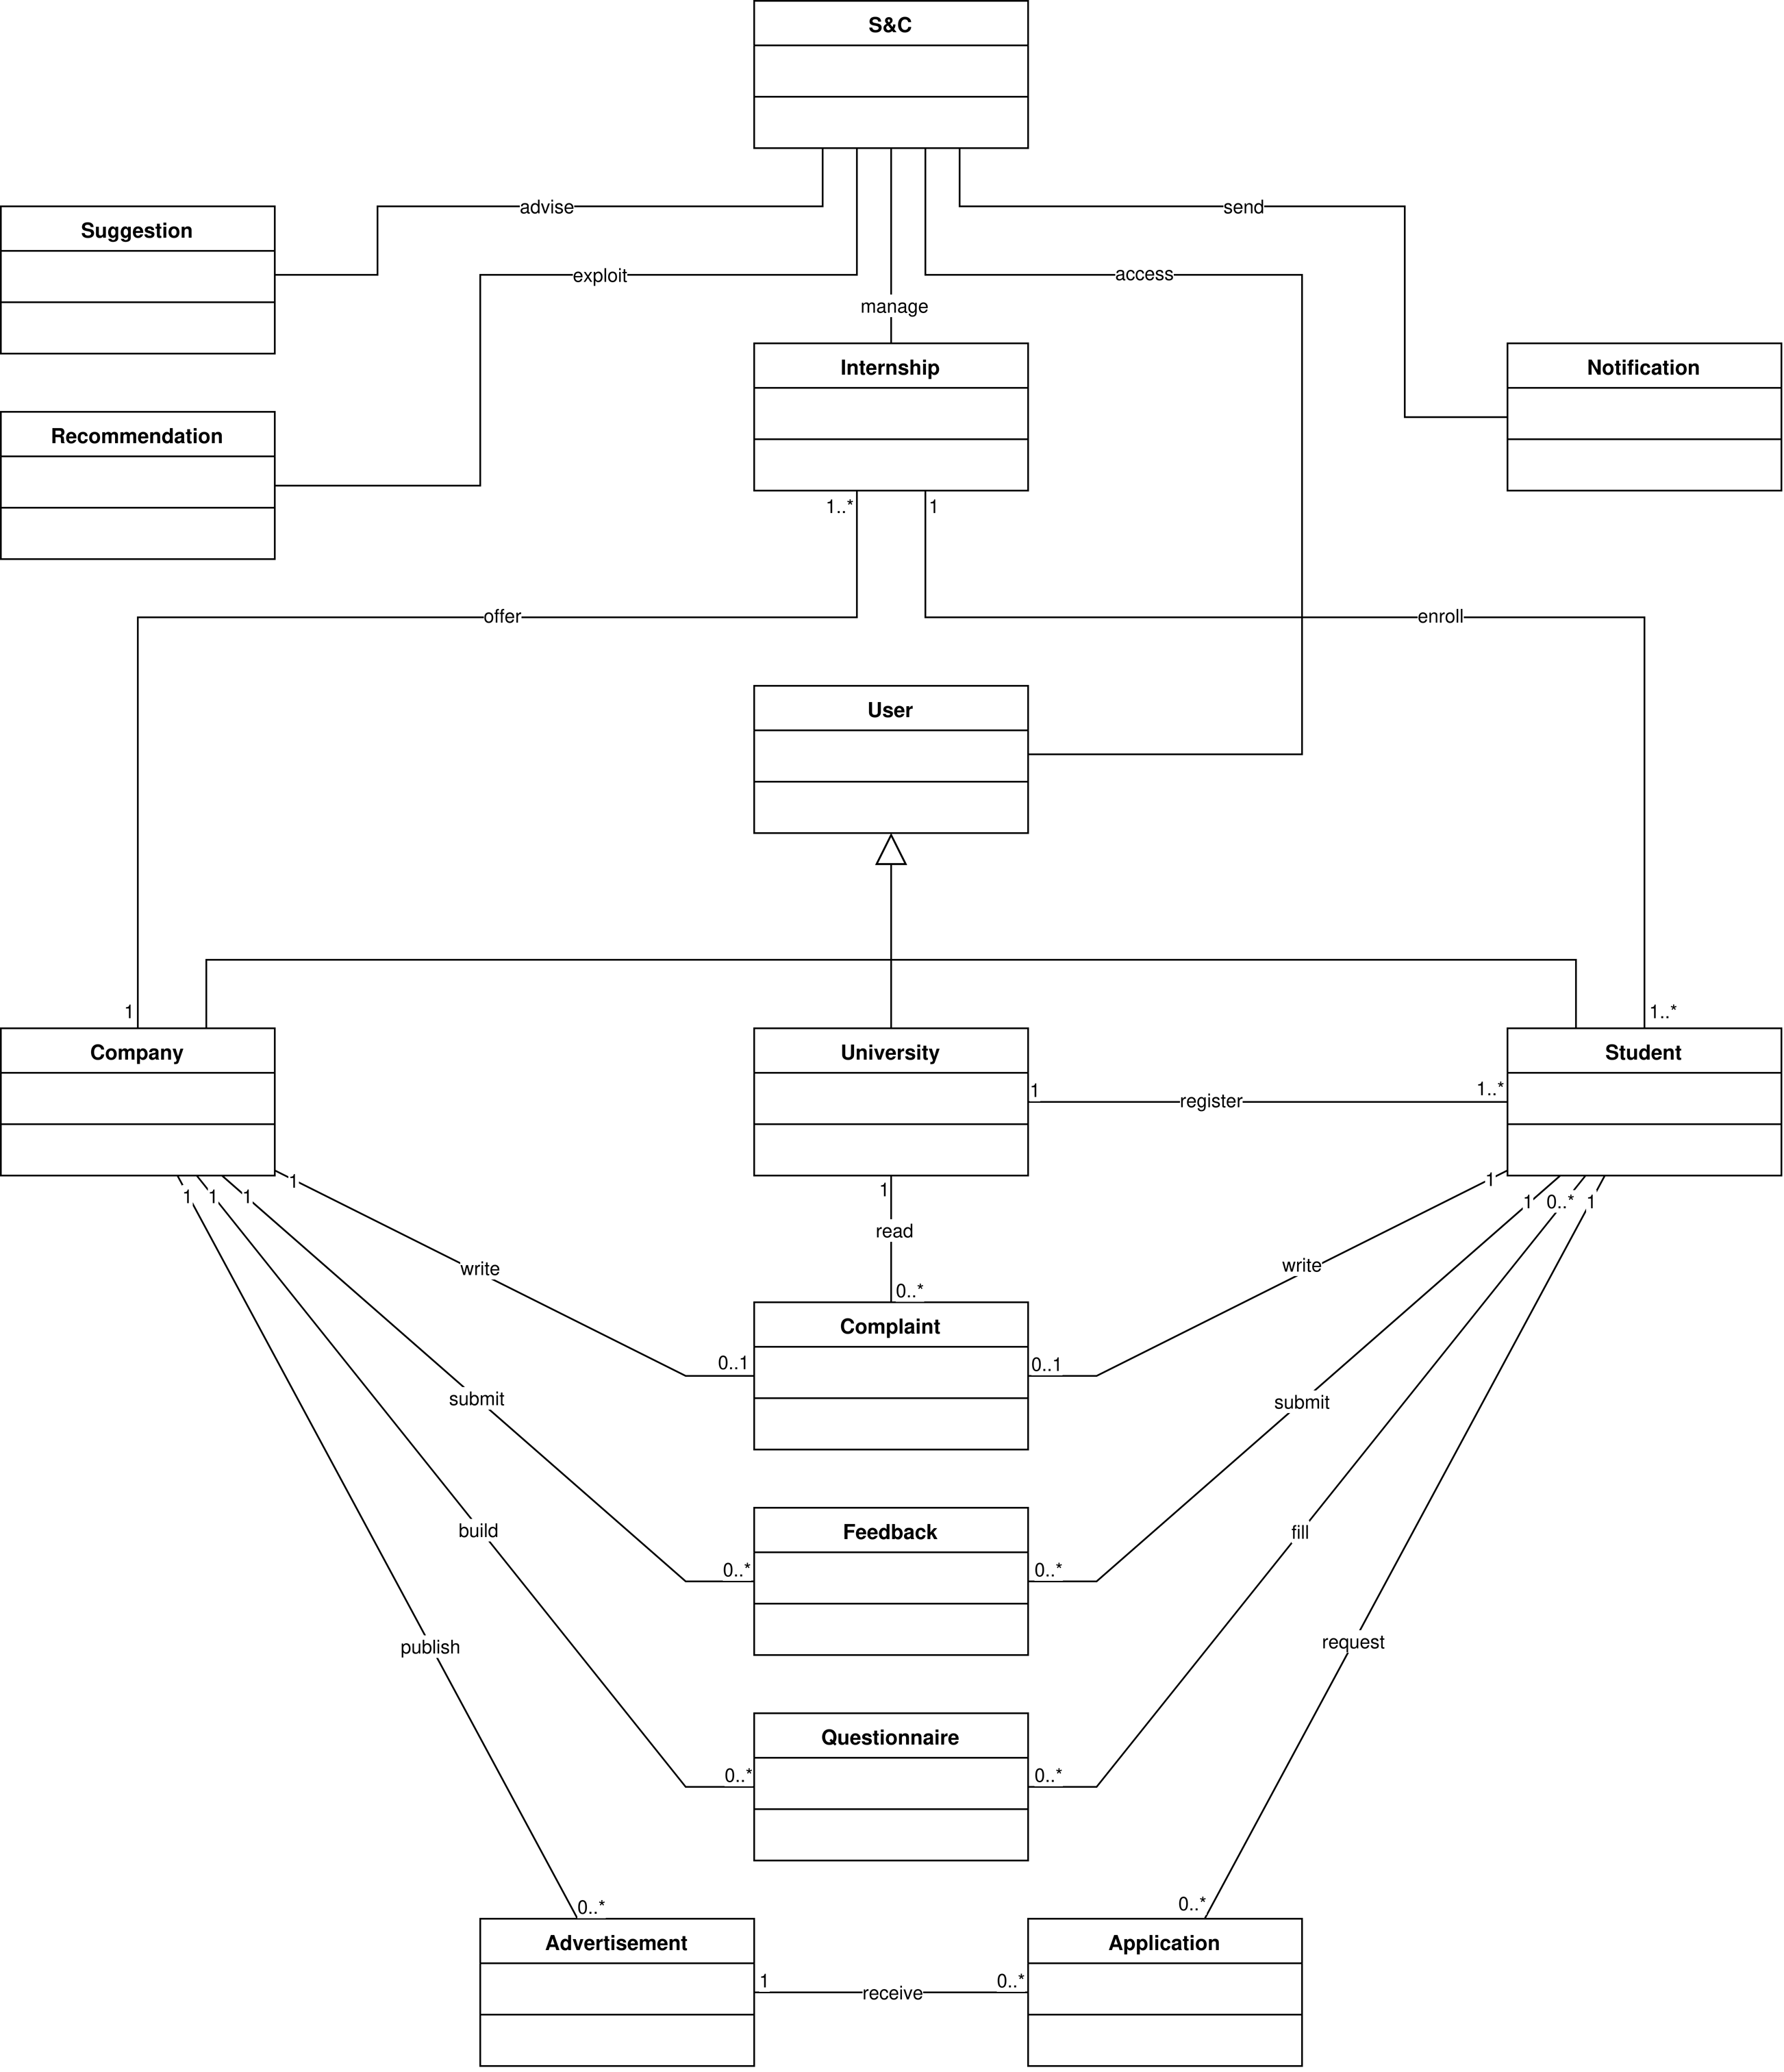
\includegraphics[width=0.8\linewidth]{../assets/class-diagrams/SC-UML.png}
\end{figure}

\subsection{State charts}

\subsubsection{Selection process}

The selection process comprehends all the actions that the student and the company take, from looking for advertisements to filling in and submitting the questionnaire.

\begin{figure}[H]
    \centering
    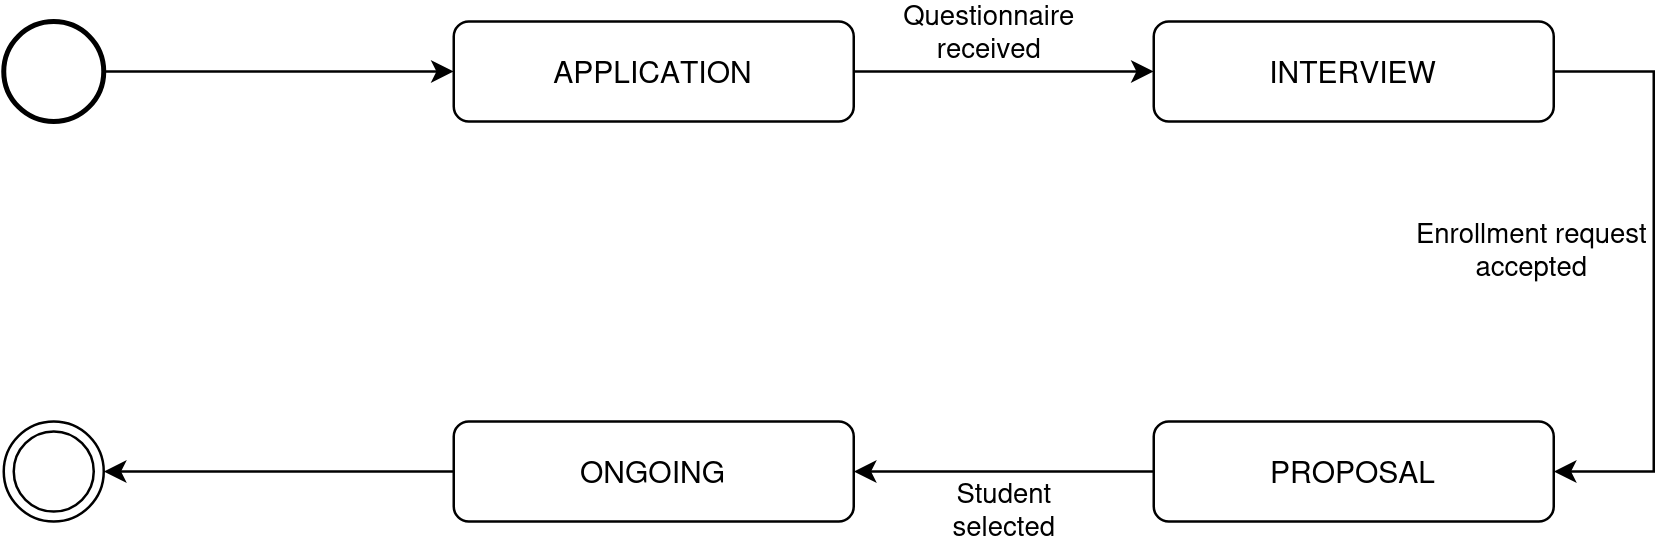
\includegraphics[width=0.8\linewidth]{../assets/state-charts/selection-process.png}
\end{figure}

\subsubsection{Complaints addressing}

Complaints are sent to the university by students and companies, and if the issue cannot be addressed and solved, the ongoing internship is interrupted.

\begin{figure}[H]
    \centering
    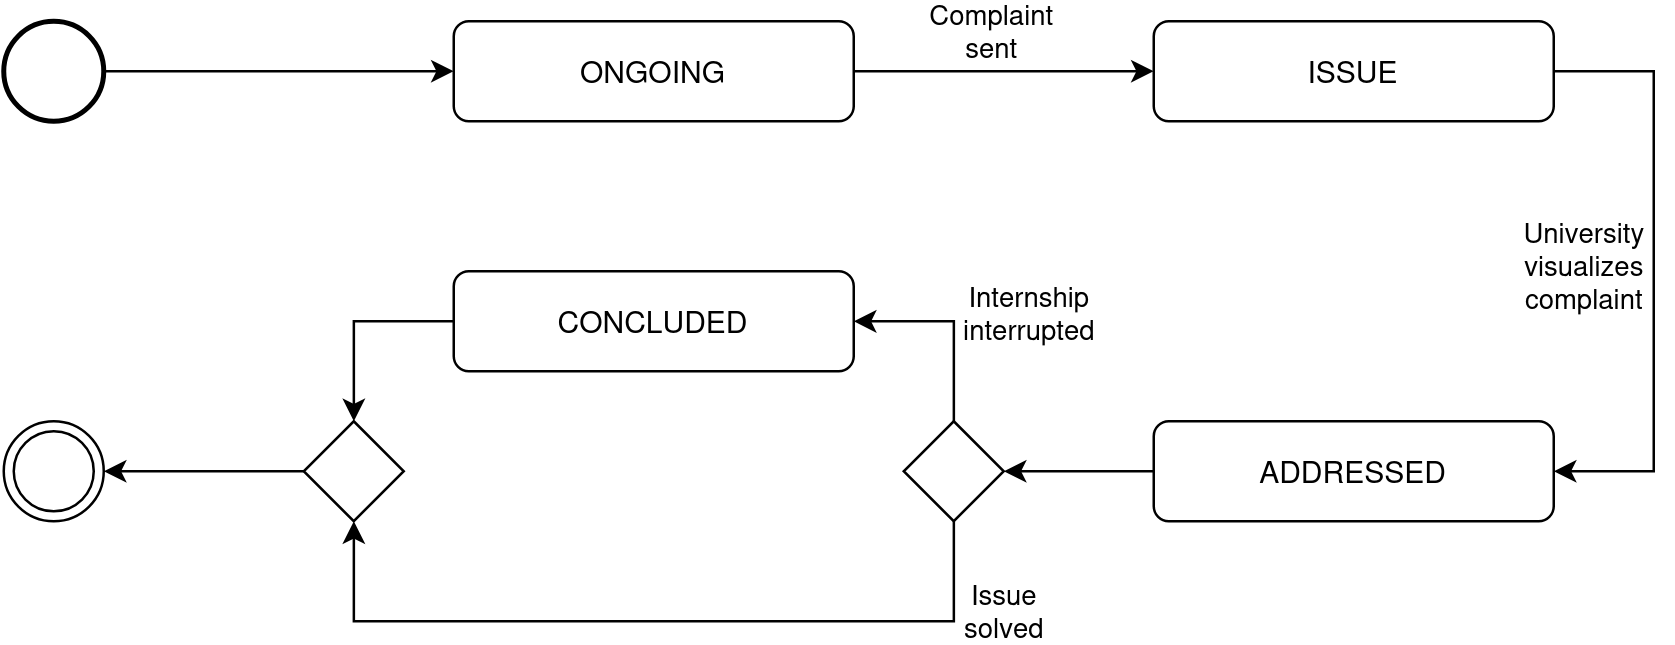
\includegraphics[width=0.8\linewidth]{../assets/state-charts/complaints-addressing.png}
\end{figure}

\subsubsection{Feedback collection}

After the internship is concluded, either because it expired or due to arising issues, the system prompts the participants to fill in and submit a feedback form, in order to collect information regarding the internship.

\begin{figure}[H]
    \centering
    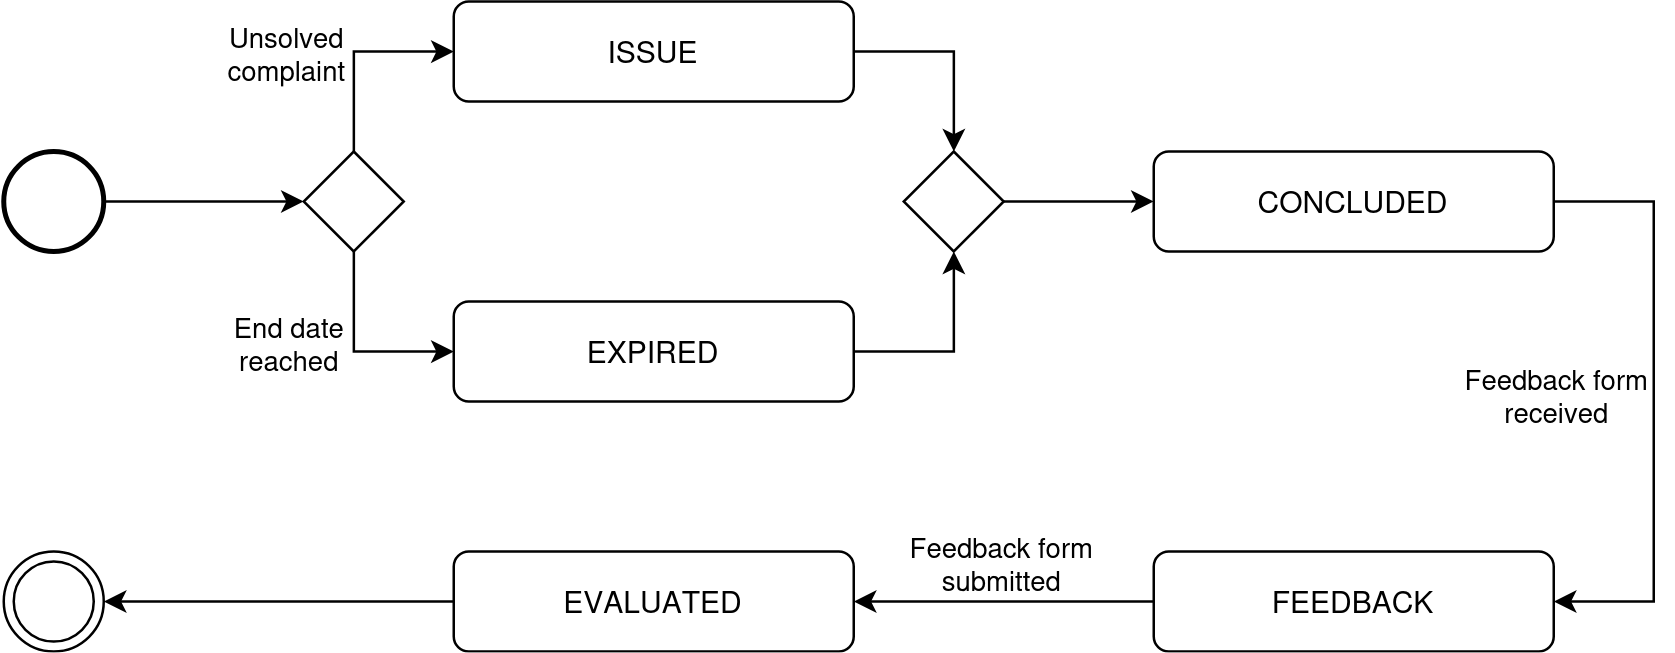
\includegraphics[width=0.8\linewidth]{../assets/state-charts/feedback-collection.png}
\end{figure}

\section{Product functions}

\subsection{Key functions}

\begin{enumerate}[label=\textbf{KF\arabic* -}]
    \item \textbf{Internship project advertisements -}
    Companies can post detailed internship project descriptions, including tasks, required skills, technologies, and terms like compensation and benefits.
    This provides students clear insights about the available opportunities.
    \item \textbf{CV upload -}
    Students can upload and manage their CVs, listing skills, experiences, and interests.
    This helps the system match students with suitable internships and allows companies to view candidate profiles.
    \item \textbf{Interviews via custom questionnaires -}
    S\&C supports the interview process by allowing companies to set up structured questionnaires, enabling them to gather specific information from candidates and assess their compatibility with the internship.
    \item \textbf{Complaints management -}
    The platform includes a complaints management feature where students and companies can report issues to the university, that can then address is accordingly, ensuring smooth and fair handling of internship-related problems.
    \item \textbf{Recommendation system -}
    S\&C employs a recommendation system that connects students with internships based on CV content and project requirements, using keyword matching statistical analyses, to optimize matches.
    \item \textbf{Suggestion system -}
    The platform provides guidance for students and companies on improving their CVs and project descriptions, enhancing their appeal and increasing the likelihood of successful matches.
\end{enumerate}

\subsection{Requirements}

\begin{enumerate}[label=\textbf{R\arabic* -}]
    \item The system must allow an unregistered student to sign up.
    \item The system must allow an unregistered company to sign up.
    \item The system must allow an unregistered university to sign up.
    \item The system must allow a registered user to log in.
    \item The system must allow a registered user to fill in and edit its personal information.
    \item The system must allow a registered student to upload its CV.
    \item The system must allow a registered company to post an internship project.
    \item The system must allow a registered student to visualize a list of open internship projects.
    \item The system must allow a registered company to visualize a list of eligible students.
    \item The system must allow a registered student to make an enrollment request to an internship project.
    \item The system must allow a registered company to build custom made questionnaires.
    \item The system must allow a registered company to send questionnaires to students.
    \item The system must allow a registered student to fill in the questionnaire.
    \item The system must allow a registered company to accept students enrollment requests.
    \item The system must allow a registered student to see their ongoing internship information.
    \item The system must allow a registered company to see their ongoing internships information.
    \item The system must allow a registered university to see their students ongoing internship information.
    \item The system must allow a registered student to send complaints to the university.
    \item The system must allow a registered company to send complaints to the university.
    \item The system must allow a registered university to visualize complaints it received.
    \item The system must allow a registered university to end an ongoing internship of its student.
    \item The system must allow a registered student to fill in a feedback form when the internship ends.
    \item The system must allow a registered company to fill in a feedback form when the internship ends.
    \item The system must allow a registered student to visualize a list of suggested internships.
    \item The system must allow a registered company to visualize a list of suggested students.
    \item The system must allow a registered student to be notified about recommended internship.
    \item The system must allow a registered company to be notified about recommended students.
\end{enumerate}

\section{User characteristics}

\htitle{Student}
Students actively seek internships to gain practical experience.
They create profiles and upload CVs, detailing their skills, experiences, and interests.
Students can proactively search for internships, receive recommendations for suitable roles, and engage in the selection process.
They can also provide feedback on internships and report any issues through the platform.

\htitle{Company}
Organizations look for interns to hire for specific projects.
They use the platform to post internship opportunities, specifying requirements like skills, tasks, and technologies.
Companies receive recommendations for matching candidates, review CVs, conduct interviews via custom questionnaires, and can provide feedback on the internship experience.
They can also provide feedback or report issues with interns.

\htitle{University}
Academic institutions oversee student internships to ensure they align with educational standards.
Universities monitor internship statuses, handle critical complaints that may require intervention, providing support if internships issues arise.
They play a supervisory role to ensure students benefit from safe, constructive, and academically relevant internship experiences.

\section{Assumptions, dependencies and constraints}

This section serves as a comprehensive overview of critical factors which must be considered during the implementation of the platform.
It consolidates the foundational assumptions made during project planning and highlights eventual dependencies.

\subsection{Domain assumptions}

\begin{enumerate}[label=\textbf{D\arabic* -}]
    \item The user must have a working internet connection.
    \item The user must have provided valid personal information.
    \item The student must be registered to a university.
    \item The university must have provided an organization mail to the student.
    \item The university must have been registered in the system directly by a staff member.
\end{enumerate}

\subsection{Dependencies}

For the registration process, a verification email must be sent by the system to the user, to successfully
sign up.
This action requires the integration of an email service.

